% documentclass
% set font size=11 (11pt)
% set paper format=A4 (a4paper)
% set equation alignment to left (fleqn)
\documentclass[11pt,a4paper,fleqn]{article}


% Preamble
% use the inputenc and fontenc packages to use French accents
\usepackage[utf8]{inputenc}
\usepackage[T1]{fontenc}
% for matrices / vectors
\usepackage{amsmath}
% for references
\usepackage{hyperref}
% allow for arbitrary font size
\usepackage{anyfontsize}
% for color
\usepackage{xcolor}
% for pseudocolor
\usepackage{algorithm,algpseudocode}
% for code samples
\usepackage{listings}
% set the font as Time New Roman (the Latex equivalent, at least)
% \usepackage{mathptmx}
% set the size of the document margins using the geometry package
\usepackage[lmargin=0.97in,rmargin=0.97in,tmargin=1.4in,bmargin=1.4in]{geometry}
% turn the color of footnote markers to black
\renewcommand\thefootnote{\textcolor{black}{\arabic{footnote}}}
% suppress indents on footnotes
\usepackage[hang,flushmargin]{footmisc}
% automatically generates colored brackets around references
\usepackage{fncylab} \labelformat{equation}{(#1)}
% supress indent on new paragraphs
\setlength{\parindent}{0pt}
% use the amsmath package to include mathematical symbols
\usepackage{amsmath}
% suppress the space between the left margin and the equations (fleqn still leaves some space by default)
\setlength{\mathindent}{0pt}
% create a new environment to left flush the equation with the align environment
\makeatletter
\newenvironment{lflalign}{ \vspace{-3mm}%
  \def\align@preamble{%
    &\strut@
    \setboxz@h{\@lign$\m@th\displaystyle{####}$}%
    \ifmeasuring@\savefieldlength@\fi
    \set@field
    \hfil
    \tabskip\z@skip
    &\setboxz@h{\@lign$\m@th\displaystyle{{}####}$}%
    \ifmeasuring@\savefieldlength@\fi
    \set@field
    \hfil
    \tabskip\alignsep@
  }
  \flalign}
{\endflalign}
\makeatother
% use the ammssymb package to use mathematical symbols
\usepackage{amssymb}
% create new commands for mathematical symbols
\DeclareMathOperator{\N}{\mathbb{N}}
\DeclareMathOperator{\Z}{\mathbb{Z}}
\DeclareMathOperator{\Q}{\mathbb{Q}}
\DeclareMathOperator{\R}{\mathbb{R}}
\DeclareMathOperator{\Pb}{\mathbb{P}}
% declare the cmsy (computer modern symbol) math alphabet to define appropriate fonts for the U and N mathematical symbols
\DeclareMathAlphabet\mathbcal{OMS}{cmsy}{m}{n}
% create new commands for mathematical symbols
\DeclareMathOperator{\E}{\mathbcal{E}}
\DeclareMathOperator{\Ex}{\mathbb{E}}
\DeclareMathOperator{\F}{\mathbcal{F}}
\DeclareMathOperator{\G}{\mathbcal{G}}
\DeclareMathOperator{\M}{\mathbcal{M}}
\DeclareMathOperator{\HH}{\mathbcal{H}}
\DeclareMathOperator{\QQ}{\mathbcal{Q}}
\DeclareMathOperator{\PP}{\mathbcal{P}}
\DeclareMathOperator{\Noo}{\mathbcal{N}}
\DeclareMathOperator{\U}{\mathbcal{U}}
% use the bbm package to be able to use the double stroke 1 for the indicator function
\usepackage{bbm}
\DeclareMathOperator{\ind}{\mathbbmss{1}}
% use the bm package to use bold characters in math mode
\usepackage{bm}
% create a new command for black square bullets
\newcommand{\bs}{\scalebox{0.7}{$\blacksquare$} \hspace{2mm}}
% use the relsize package to be abe to change the size of mathematical symbols
\usepackage{relsize}
% define a new command for in-line small summation
\newcommand{\ssumm}[2]{\underset{\scriptscriptstyle #1}{\overset{\scriptscriptstyle #2}{\mathlarger{\mathlarger{\mathlarger{\Sigma}}}}} \hspace{0.5mm}}
% define a new command for in-line small products
\newcommand{\sprod}[2]{\underset{\scriptscriptstyle #1}{\overset{\scriptscriptstyle #2}{\mathlarger{\mathlarger{\mathlarger{\Pi}}}}} \hspace{0.5mm}}
% Use the caption package to customize captions (titles) of tables and graphs
\usepackage[font=small,labelfont=bf]{caption}
% use float package to force figure the be positioned where indicated
\usepackage{float}
% use the graphicx package to be able to resize tables
\usepackage{graphicx}


\begin{document}

% command to check unused bibliography entries
% \nocite{*}
{\fontsize{20pt}{22pt}\selectfont \textbf{Theory} \par}
\vspace{10mm}
{\fontsize{12pt}{22pt} \textbf{Bayes classifier}\par}

\vspace{5mm}

$g$ is the \textit{classifier}.

$$g: \mathcal{X} \to \mathcal{Y}$$
$$~~~~~~~~~~\mathbb{R}^d \to \{0,1\}$$

To model the learning problem, we use the pair $(X,Y)$ described by $(\mu, \eta)$ where $\mu$ is the probability measure:

$$\mu(A) = \mathbb{P}(X \in A)$$

And $\eta$ is the regression of $Y$ on $X$:

$$\eta(X) = \mathbb{P}(Y=1 | X=x) = \mathbb{E}[Y | X=x]$$

$\eta$ is also called the \textit{a posteriori probability}.

The Bayes classifier is:

  \begin{equation}
    \begin{cases}
      1 & \text{if}\ \eta(x) > 1/2 \\
      0 & \text{otherwise}
    \end{cases}
  \end{equation}

Or, if $\mathcal{Y}$ is $\{-1,1\}$, we write the classifier as such: $g(x) = 2 \mathbbm{1}\{ \eta(x)>1/2\}-1$.

\vspace{5mm}

\underline{Theorem}:

\vspace{5mm}

For any classifier g: $\mathbb{R}^d \to \{0,1\}$,
$$\mathbb{P}(g^*(X) \neq Y) \le \mathbb{P}(g(X) \neq Y)$$

In other words, the Bayes classifier is theorically \textbf{the best classifier}.

\vspace{5mm}

\textit{Proof}: express $\mathbb{P}(g(X) \neq Y) - \mathbb{P}(g^*(X) \neq Y)$ in terms of dummies (use complementaries) and show that it is superior to 0.

\vspace{5mm}
{\fontsize{12pt}{22pt} \textbf{Gradient descent}\par}

\vspace{5mm}

$\ell$ the loss function to minimize:

$\theta_{t+1}=\theta_t - \alpha \nabla \ell$ \\

\begin{algorithm}
\caption{Global gradient descent}
\begin{algorithmic}
\State Loss function $\widehat{L}_n(\hat{f}_\omega(x))=\Sigma_{i=1}^n \mathcal{\ell}(\hat{f}_\omega(x),y)$
\State $E=1000$
\State $\epsilon$ = small value
\State $\omega_0$ = intial value in $t_0$
\While{$E > \epsilon$}
\State $\omega_{t+1}=\omega_t-\epsilon\Sigma_{i=1}^n\nabla_\omega{\mathcal{\ell}(\hat{f}_\omega(x),y)}$
\State Compute $E=L_n(\omega_{t+1})$
\EndWhile
\end{algorithmic}
\end{algorithm}


\begin{algorithm}
\caption{Stochastic gradient descent}
\begin{algorithmic}
\State Loss function $\widehat{L}_n(\hat{f}_\omega(x))=\Sigma_{i=1}^n \mathcal{\ell}(\hat{f}_\omega(x),y)$
\State $E=1000$
\State $\epsilon$ = small value
\State $\omega_0$ = intial value in $t_0$
\While{$E > \epsilon$}
\For{i = 1,...,n}
\State $\omega_{t+1}=\omega_t-\epsilon\nabla_\omega{\mathcal{\ell}(\hat{f}_\omega(x_i),y_i)}$
\State Compute $E=L_n(\omega_{t+1})$
\EndFor
\EndWhile
\end{algorithmic}
\end{algorithm}

\begin{algorithm}
\caption{Stochastic and random gradient descent}
\begin{algorithmic}
\State Loss function $\widehat{L}_n(\hat{f}_\omega(x))=\Sigma_{i=1}^n \mathcal{\ell}(\hat{f}_\omega(x),y)$
\State $E=1000$
\State $\epsilon$ = small value
\State $\omega_0$ = intial value in $t_0$
\While{$E > \epsilon$}
\For{i = 1,...,n}
\State Random draw of $i \in \{1,...,n\}$
\State $\omega_{t+1}=\omega_t-\epsilon\nabla_\omega{\mathcal{\ell}(\hat{f}_\omega(x_i),y_i)}$
\State Compute $E=L_n(\omega_{t+1})$
\EndFor
\EndWhile
\end{algorithmic}
\end{algorithm}

\vspace{30mm}

The main advantage of stochastic gradient is that it avoid computing the gradient descent on all the observations (greedy). However, in doing so, the gradient descent is subject to noise and can take longer to reach the optimum. \\

\textit{Note}: the gradient is the derivation w.r.t $\omega$

\textit{Note (stochastic and random gradient descent)}: the draw can be done with or without replacement. \\



\underline{Proof of the gradient descent formula}:

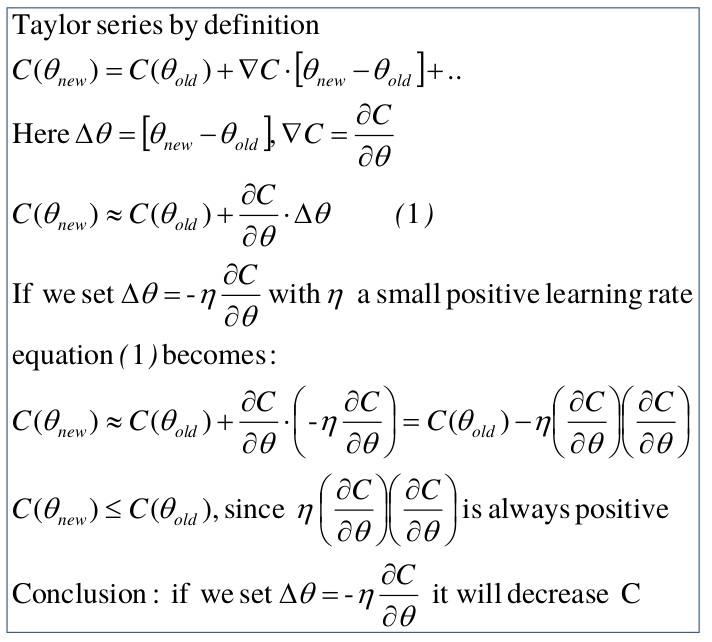
\includegraphics[scale=0.3]{../images/GradientDescent_proof.png}

(Idemia courses "DeepLearningTPT2018S1S2.pdf")

\vspace{5mm}
\underline{Learning rate optimization}
\vspace{5mm}

Note:

- one epoch = one forward pass and one backward pass of all the training examples.

- batch size = the number of training examples in one forward/backward pass. The higher the batch size, the more memory space needed.

- number of iterations = number of passes, each pass using [batch size] number of examples. To be clear, one pass = one forward pass + one backward pass.

\vspace{5mm}

\textit{Learning rate decay}

Simple idea: reduce the learning rate progressively.

E.g. $1/t$ decay:

$$\alpha_t=\frac{1}{(t+1)}$$

\vspace{5mm}
\textit{Momentum}

Momentum is a method that helps accelerate SGD in the relevant direction and reduce oscillations.

General idea:

$0 \le \gamma \le 1$

$M_{t_0}=x_0$

$M_{t_1}=\gamma M_{t_0} + x_1$

$M_{t_2}=\gamma M_{t_1} + x_2$

Let's develop $M_{t_2}$ to have a better view of momentum effect:

$M_{t_2} = \gamma (\gamma M_{t_0} + x_1) + x_2 = \gamma^2 x_0 + \gamma x_1 + x_2$

We can see that more importance is given to the most recent value ($x_2$) and the least to the past values.

\vspace{5mm}

In practice, $\gamma = 0.9$ gives good results.

\textbf{Advantage}: less dependent on noise

\vspace{5mm}
\textit{Adagrad - Adaptive Gradient Algorithm (2011)}

Divide the learning rate by "average" gradient:

$\theta_t = \theta_{t-1} - \frac{\alpha}{\sqrt{\Sigma_{i=0}^t(\nabla f_i^2)}}\nabla f$

\vspace{5mm}
\textit{RMSProp - Root Mean Squared Propagation}

Same as AdaGrad, but with an exponentially decaying average of past squared gradients.

$\theta_t = \theta_{t-1} - \frac{\alpha}{\sigma_{t-1}}\nabla f$

Where:

$\sigma_{t} = \sqrt{\alpha (\sigma_{t-1})^2+(1-\alpha)(\nabla f_t)^2}$


\vspace{5mm}
\textit{Adam - Adaptive moment estimation}

Adam = RMS + momentum => use of a exponential decaying average of past \underline{squared} gradients and past gradients

\vspace{5mm}
\section*{Bias-Complexity trade-off}

\label{sec:bias-complexity-trade-off}

\vspace{5mm}

$ERM$ = Empiric Risk Minimization algorithm

$\mathcal{H}$ = hypothesis class = all the classifiers that are considered

\vspace{5mm}

We can decompose the error of an $ERM_\mathcal{H}$:

$$L_{\mathcal{D}}(h_s) = \epsilon_{app} + \epsilon_{est}$$

- \textit{Approximation error}: $\epsilon_{app} = min_{h \in \mathcal{H}} L_{\mathcal{D}}(h)$. This is the error done by the best predictor among those considered.

- \textit{Estimation error}: $\epsilon_{est} = L_{\mathcal{D}}(h) - \epsilon_{app}$. This is the error difference from a used predictor and the best one.

$\epsilon_{app}$ low => $\epsilon_{est}$ high => overfitting

$\epsilon_{est}$ low => underfitting

\vspace{5mm}
{\fontsize{20pt}{22pt}\selectfont \textbf{Supervised learning} \par}
\vspace{10mm}
Supervised learning aims at \textbf{finding a predictor when we have data with their labels}.

\vspace{5mm}
{\fontsize{12pt}{22pt} \textbf{Logistic regression}\par}

\vspace{5mm}

Logistic regression is used for binary classification.

It is quite similar to a simple linear regression in the sense that the objective is to find optimal weights $\omega$ to predict a variable. However, in the logistic regression we use a sigmoïd function.\\

Rem: "logistic" because the logistic law has a sigmoïd function as a repartition function.\\

\underline{Rationale behind the use of the sigmoïd function}:

We look for the \textit{à posteriori} probability $\mathbb{P}(x | y=1) = \pi (x) = \hat{y}$.

The predicted variable $\hat{y}$ is thus a probability.  \\

The sigmoïd function: $\sigma: z \to \frac{1}{1+e^{-z}}$ is well adapted because we want an output that is included in $[0,1]$.

\begin{center}
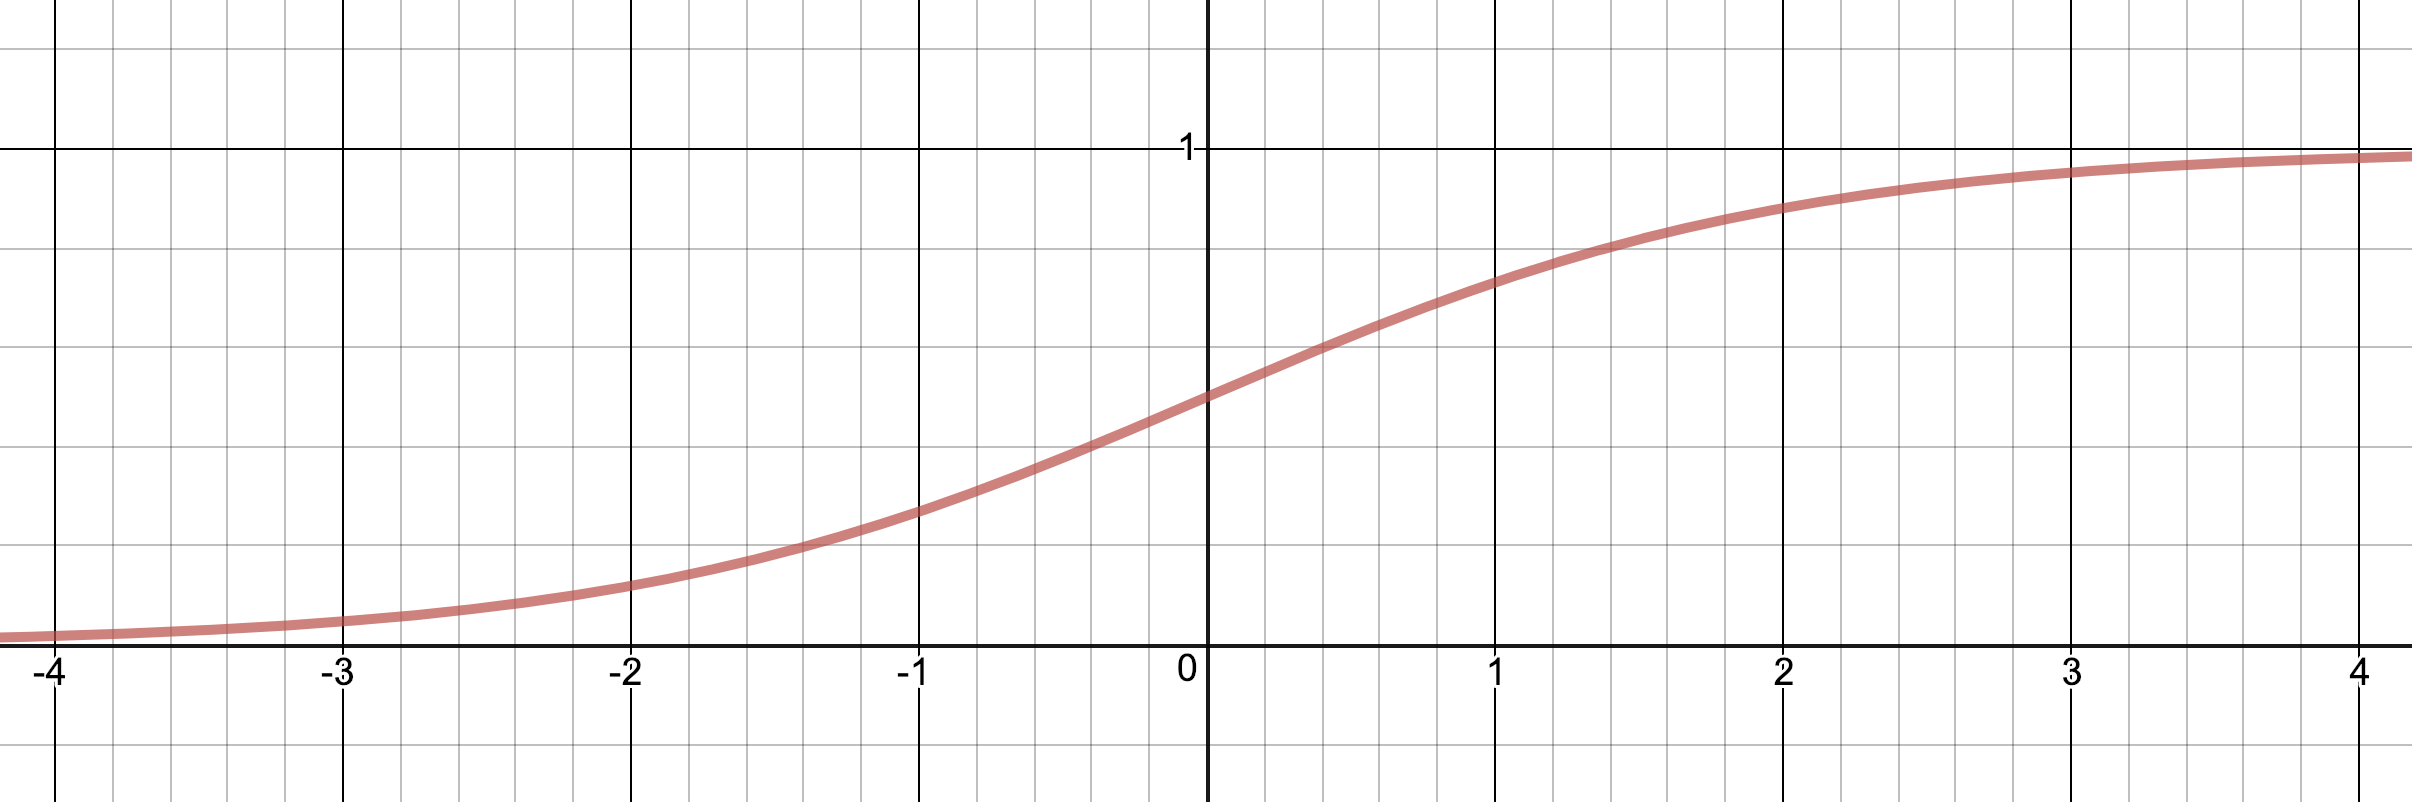
\includegraphics[scale=0.15]{sigmoid.png}
\end{center}

Classification function: $\widehat{f}_{\omega}(x) = \sigma(\omega x)$ with a threshold \\

\underline{Loss function}

If $y = 1$, we want $\sigma(\omega x)$ to be high => $1 - \sigma(\omega x)$ should be low. The loss function should be increasing with $1 - \sigma(\omega x) = 1 - \frac{1}{1+e^{-\omega x}} = \frac{1}{1+e^{\omega x}}$. Equivalently, it should be increasing with $1 + e^{-\omega x}$.

More generally, the loss function is defined as such: $\ell(f_{\omega}, (x,y)) = log(1 + e^{-y \omega x})$ (adding $y$ in the expression allows to take into account cases when $y = 1$ and $y = -1$).

Recall that the log is a monotonic function.

\vspace{5mm}

\underline{Estimation}

The advantage of the logistic loss function is that it is a convex function. Hence the ERM problem can be solved efficiently using standard methods.

Estimation is done using maximum likelihood. Maximum likelihood is finding the parameter that maximizes the probability to have a specific event $(x_i, y_i)$. We want to maximize the \textit{à posteriori} probability that depends on $x$: \\

$L(\omega, b) = \prod_{i=1}^n \pi(x_i)^{y_i}(1-\pi(x_i))^{1-y_i}$ \\

This equation has no analytic solution. We use a numeric method to find the optimal parameters (see optimizaton algorithms).

See \textit{Neural Network} section for more details on optimization.

\vspace{5mm}

Note: logistic regression is really a linear model since the objective is to find $\omega$ that is the slope of the line $\omega ^Tx + b$.

\vspace{5mm}
{\fontsize{12pt}{22pt} \textbf{Linear discriminant analysis}\par}

\vspace{5mm}

We focus on the binary case, that is when $Y=+1$ or $Y=-1$, that is to sets of variables.

These two conditional laws need to be gaussians with same covariance: \vspace{1mm}

$X | Y=+1 \sim \mathcal{N}(\mu_+,\Sigma)$ with density $f_+$

$X | Y=-1 \sim \mathcal{N}(\mu_-,\Sigma)$ with density $f_-$

Let $\pi_+$, $\pi_-$ be the simple probabilities $P(Y=+1)$, $P(Y=-1)$\vspace{3mm}

$ \mathbb{P}\{Y=+1|X=x\} = \frac{\mathbb{P}\{Y=+1, X=x\}}{\mathbb{P}\{X=x\}}$

$ \mathbb{P}\{Y=+1|X=x\} = \frac{\mathbb{P}\{X=x|Y=+1\} \mathbb{P}\{Y=+1\} }{\mathbb{P}\{X=x\} }$

$ \mathbb{P}\{Y=+1|X=x\} = \frac{f_+ \pi_+}{\mathbb{P}\{X=x\} }$

$ \mathbb{P}\{Y=+1|X=x\} = \frac{f_+ \pi_+}{(\mathbb{P}\{X=x|Y=+1\}\mathbb{P}\{Y= +1\} + \mathbb{P}\{X=x|Y=-1\}\mathbb{P}\{Y= -1\}) }$

$\mathbb{P}\{Y=+1|X=x\} = \frac{f_+ \pi_+}{(f_+\pi_+ + f_-\pi_-)}$

Similarly,

$ \mathbb{P}\{Y=-1|X=x\} = \frac{f_- (1-\pi_+)}{\mathbb{P}\{X=x\} }$

$\mathbb{P}\{Y=-1|X=x\} = \frac{f_- (1-\pi_+)}{(f_+\pi_+ + f_-\pi_-)}$

\vspace{3mm}

The result shows us that we can express the two conditionnal probabilities in terms of conditionnal densities and "simple" probabilities ($\pi_+$, $\pi_-$).

Recall that multivariable gaussian density is: $f(x)=\frac{1}{\sqrt{2 \pi |\Sigma|}}e^{-\frac{1}{2}(x-\mu)^T\Sigma^{-1}(x-\mu)}$

In practice, $\mu_+$, $\mu_-$, $\pi_+$ and $\Sigma$ are unknown. Thus we use empiric values:

$\widehat{\pi}_+ = m/n$

$\widehat{\mu}_+ = \frac{1}{m} \Sigma \mathbbm{1}_{\{y_i=+1\}}x_i$

$\widehat{\mu}_- = \frac{1}{n-m} \Sigma \mathbbm{1}_{\{y_i=-1\}}x_i$

$\widehat{\Sigma} = \frac{1}{n-2} ((m-1) \widehat{\Sigma}_+ + (n-m-1)\widehat{\Sigma}_-)$

$\widehat{\Sigma}_+ = \frac{1}{m-1} \Sigma \mathbbm{1}_{\{y_i=+1\}}(x_i-\widehat{\mu}_+)(x_i-\widehat{\mu}_+)^T$

$\widehat{\Sigma}_- = \frac{1}{n-m-1} \Sigma \mathbbm{1}_{\{y_i=-1\}}(x_i-\widehat{\mu}_-)(x_i-\widehat{\mu}_-)^T$

 \vspace{3mm}

\underline{Classification}

We predict class = 1 when $\mathbb{P}(Y=+1 | X) > \mathbb{P}(Y=-1 | X)$

=> $\frac{\mathbb{P}(Y=+1 | X)}{\mathbb{P}(Y=-1 | X)} > 1$

=> $\log(\frac{\mathbb{P}(Y=+1 | X)}{\mathbb{P}(Y=-1 | X)}) > 0$

=> 

Using previous conditional probability expressions, we end up with the following prediction rule:

  \begin{equation}
    \begin{cases}
      1 & \text{if}\ x^T\widehat{\Sigma}^{-1}(\widehat{\mu}_+ - \widehat{\mu}_-) > \frac{1}{2}\widehat{\mu}_+^T\widehat{\Sigma}\widehat{\mu}_+ - \frac{1}{2}\widehat{\mu}_-^T\widehat{\Sigma}\widehat{\mu}_- + \log(1-m/n) - \log(m/n) \\
      -1 & \text{otherwise}
    \end{cases}
  \end{equation}

$\widehat{\mu}_+$, $\widehat{\mu}_-$, $\widehat{\pi}_+$ and $\widehat{\Sigma}$ will be computed with \textit{train data}.

 $x$ is the \textit{test data}.

\vspace{3mm}

\textit{Note}: $\widehat{\Sigma}^{-1}(\widehat{\mu}_+ - \widehat{\mu}_-)$ is the \textbf{Fisher function} (Saporta).

\lstset{language=Python}
\lstset{frame=lines}
\lstset{caption={LDA algorithm}}
\lstset{label={lst:code_direct}}
\lstset{basicstyle=\footnotesize}
\begin{lstlisting}

class LDAClassifier():
    
    def fit(self, X, y):       
        
        X_p = X[y == 1, :]
        X_m = X[y == -1, :]
        
        X_p_x1 = X_p[:,0]
        X_p_x2 = X_p[:,1]
        X_m_x1 = X_m[:,0]
        X_m_x2 = X_m[:,1]
        
        n = len(X)
        m = len(X_p)
        
        mean_p_x1 = np.mean(X_p_x1)
        mean_p_x2 = np.mean(X_p_x2)
        mean_p = np.array([mean_p_x1,mean_p_x2]) # mu_plus (estimated)
        cov_p = np.cov(np.transpose(X_p))
        

        mean_m_x1 = np.mean(X_m_x1)
        mean_m_x2 = np.mean(X_m_x2)
        mean_m = np.array([mean_m_x1,mean_m_x2]) # mu_minus (estimated)
        cov_m = np.cov(np.transpose(X_m))
        
        cov_est = (1/(n-2))*( (m-1)* cov_p + (n-m-1)* cov_m) # sigma (estimated)
        inv_cov_est = np.linalg.inv(cov_est)
        
        a1 = np.dot(np.transpose(mean_p),inv_cov_est)
        a2 = np.dot(np.transpose(mean_m),inv_cov_est)
        
        # 2nd term in inequality
        self.alpha = 0.5*(np.dot(a1,mean_p)  - 0.5*np.dot(a2,mean_m)) + np.log(1- m/n) - np.log(m/n)
        # 1st term in inequality
        self.beta =  np.dot(inv_cov_est,mean_p-mean_m)
        
        return self
    
    def predict(self, X):
        
        y_=[]
        
        for i in range(len(X)):
            X_pred = X[i]
            beta = np.dot(np.transpose(X_pred), self.beta)
            if (beta>self.alpha):
                Y_pred = 1
            else:
                Y_pred = -1
            y_.append(Y_pred)
        return np.array(y_) 

\end{lstlisting}

\vspace{5mm}
{\fontsize{12pt}{22pt} \textbf{SVM}\par}

\vspace{5mm}

\underline{Margin}

\vspace{5mm}

This idea of SVM is to separate data as best as possible using a margin.

\begin{center}
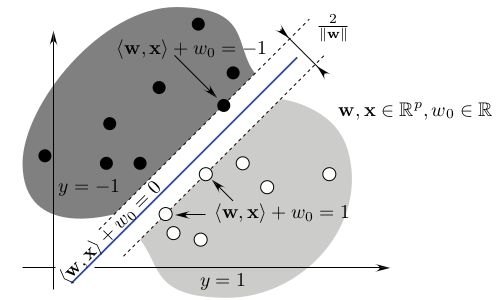
\includegraphics[scale=0.6]{SVM.png}
\end{center}

Three planes:

- $H_1: \omega^Tx+b=1$

- $H: \omega^Tx+b=0$

- $H_{-1}: \omega^Tx+b=-1$

\vspace{5mm}

Computing $H_1 - H_{-1}$ we get:

$(x_1-x_{-1})\omega^T=2$

=> $||x_1-x_{-1}||=\frac{2}{||\omega||}$

\vspace{5mm}

The SVM problem starts with a \textbf{margin maximization}. \textcolor{orange}{We want to maximize the distance between $x_1$ and $x_{-1}$ (\textbf{to be double checked})} and it is equivalent to minimizing $||\omega||$. Thus the optimization problem is written as such:

\begin{center}
$min_{\omega,b}~\frac{1}{2}||\omega||^2$

$s.t.~y_i(\omega^Tx_i+b) \geq 1$ $i=1,...,n$
\end{center}

\vspace{5mm}

\underline{Primal formulation}

\vspace{5mm}

The above problem reflects the case when all data are perfectly separable, this is not true in practice. We thus add an error term $\xi_i$ for each observation. This leads to the \textbf{primal formulation} of the problem:

\begin{center}
$min_{\omega,b, \xi}~\frac{1}{2}||\omega||^2+C\Sigma_{i=1}^{n}\xi_i$

$s.t.~y_i(\omega^Tx_i+b) \geq 1 - \xi_i$ $i=1,...,n$

$\xi_i \geq 0$ $i=1,...,n$
\end{center}

\vspace{5mm}

\textit{Note}: the problem can be rewritten with the hinge loss function

$y_i(\omega^Tx_i+b) \geq 1 - \xi_i => \xi_i \geq 1 - y_i(\omega^Tx_i+b)$

$~~~~~~~~~~~~~~~~~~~~~~~~~~~~ => \xi_i \geq 1 - y_i(\omega^Tx_i+b) \geq 0$ since $\xi_i \geq 0$

$~~~~~~~~~~~~~~~~~~~~~~~~~~~~ => \xi_i = max(0, 1 - y_i(\omega^Tx_i+b))$

$~~~~~~~~~~~~~~~~~~~~~~~~~~~~ => \xi_i = (0, 1 - y_i(\omega^Tx_i+b))_+$

$=> \xi_i = hinge(f(x))$ where $hinge$ is the \textit{Hinge loss} function 

$hinge(f(x)) = (1 - yf(x))_+$

\begin{center}
$min_{\omega,b}~\frac{1}{2}||\omega||^2+C\Sigma_{i=1}^{n} (0, 1 - y_i(\omega^Tx_i+b))_+$
\end{center}

\vspace{5mm}

\underline{Lagrange}

\vspace{5mm}

We can write this problem using Lagrange formulation, that is, integrating the constraints into the main formula:

$\mathcal{L}(\omega,b,\xi, \alpha, \mu) = \frac{1}{2}\omega^T\omega+C\Sigma \xi_i + \Sigma \alpha_i (1-\xi_i - y_i(\omega^Tx_i+b)) - \Sigma \mu_i \xi_i$

$\alpha_i, \mu_i \geq 0$

\vspace{5mm}

First order conditions:

$\frac{\partial\mathcal{L}}{\partial\omega} = 0 => \omega - \Sigma \alpha_i y_i x_i = 0 => \omega = \Sigma \alpha_i y_i x_i$

$\frac{\partial\mathcal{L}}{\partial b} = 0 => -\Sigma \alpha_i y_i = 0$

$\frac{\partial\mathcal{L}}{\partial \xi_i} = 0 => C - \alpha_i  - \mu_i = 0 => \alpha_i = C - \mu_i$

Since $\alpha_i, \mu_i \geq 0$ we have $C \geq \alpha_i \geq 0$

\vspace{5mm}

\underline{Dual formulation}

\vspace{5mm}

We can rewrite the problem using the first order conditions above:

$\mathcal{L}(\omega,b,\xi, \alpha, \mu) = \frac{1}{2}(\Sigma \alpha_i y_i x_i)^T(\Sigma \alpha_i y_i x_i)+C\Sigma \xi_i + \Sigma \alpha_i - \Sigma \alpha_i \xi_i - \Sigma \alpha_i y_i (\Sigma \alpha_i y_i x_i)^T x_i - \Sigma \alpha_i y_i b - \Sigma \mu_i \xi_i$

$~~~~~~~~~~~~~~~~~~ = -\frac{1}{2}(\Sigma \alpha_i y_i x_i)^T(\Sigma \alpha_i y_i x_i) + \Sigma(C - \alpha_i - \mu_i)\xi_i + \Sigma \alpha_i - \Sigma \alpha_i y_i b$

$~~~~~~~~~~~~~~~~~~ = -\frac{1}{2}\Sigma_{i,j} \alpha_i \alpha_j y_i y_j x_i^T x_j + \Sigma \alpha_i$

\vspace{5mm}

The problem is convex with lineary inequality constraints, we can apply the saddle point theorem.

\textit{Note}: a point is saddle if it's a maximum w.r.t. one axis and a minimium w.r.t. another axis 

The saddle theorem allows us to solve the problem $min_\omega max_\alpha$ as $max_\alpha min_\omega$

\vspace{5mm}

This leads to the problem in its \textbf{dual formulation}:

\begin{center}

$max_\alpha~~-\frac{1}{2}\Sigma_{i,j} \alpha_i \alpha_j y_i y_j x_i^T x_j + \Sigma \alpha_i$

$s.t.~~0 \leq \alpha_i \leq C~~i=1,...,n$

$\Sigma \alpha_i y_i = 0~~i=1,...,n$

\end{center}

\vspace{5mm}

Using the above expression of $\omega$ (optimal condition), the classification function is:

\begin{center}
$f(x)=sign(\Sigma \alpha_i y_i x_i^T x + b)$
\end{center}

\vspace{5mm}

\underline{Kernel}

\vspace{5mm}

Kernels are used when separation is non linear.

Recall the primal formulation:

\begin{center}
$min_{\omega,b, \xi}~\frac{1}{2}||\omega||^2+C\Sigma_{i=1}^{n}\xi_i$

$s.t.~y_i(\omega^Tx_i+b) \geq 1 - \xi_i$ $i=1,...,n$

$\xi_i \geq 0$ $i=1,...,n$
\end{center}

When separation is non linear, we set $\phi$ as a non linear transformation. The constraint becomes:

$y_i(\omega^T\phi(x_i)+b) \geq 1 - \xi_i~~i=1,...,n$

\vspace{5mm}

Dual formulation is now:

\begin{center}

$max_\alpha~~-\frac{1}{2}\Sigma_{i,j} \alpha_i \alpha_j y_i y_j \phi(x_i)^T \phi(x_j) + \Sigma \alpha_i$

$s.t.~~0 \leq \alpha_i \leq C~~i=1,...,n$

$\Sigma \alpha_i y_i = 0~~i=1,...,n$

\end{center}

\vspace{5mm}

The classification becomes:

\begin{center}
$f(x)=sign(\Sigma \alpha_i y_i \phi(x_i)^T \phi(x) + b)$
\end{center}

To classify a new point, we thus need to be able to compute $\phi(x_i)^T \phi(x)$.

\vspace{5mm}

\textbf{Kernel trick}: there is no need to know an explicit expression of $\phi$ (i.e. knowing the coordinates of points in new set) since we are only looking at distances and angles, that is scalar product.

\vspace{5mm}

Kernel functions implement those scalar products: $K(x,x')=\phi(x)^T \phi(x')$ where $\phi$ is a transformation function into a Hilbertian set $\phi : \mathcal{X} \to \mathcal{F} $

\textit{Note}: an Hilbertian is a set with scalar product: $\mathcal{F}=(\mathcal{H},<.,.>)$

\vspace{5mm}

Most used kernels:

Linear kernel: $K(x,x') = x^Tx'$ (we often call this setup a "no-kernel SVM")

Polynomial kernel: $K(x,x') = (x^Tx'+c)^d$

Gaussian kernel: $K(x,x') = exp(-\gamma||x-x'||^2)$

\vspace{5mm}

The optimisation problem can be written with kernel:

\begin{center}

$max_\alpha~~-\frac{1}{2}\Sigma_{i,j} \alpha_i \alpha_j y_i y_j K(x_i,x_j) + \Sigma \alpha_i$

$s.t.~~0 \leq \alpha_i \leq C~~i=1,...,n$

$\Sigma \alpha_i y_i = 0~~i=1,...,n$

\end{center}

\vspace{5mm}

\underline{Summary}

\vspace{5mm}

SVM allows to find complex non linear separations in transforming the problem into a higher dimension where data are linearly separable.

\vspace{5mm}

From 1D to 2D:

\begin{center}
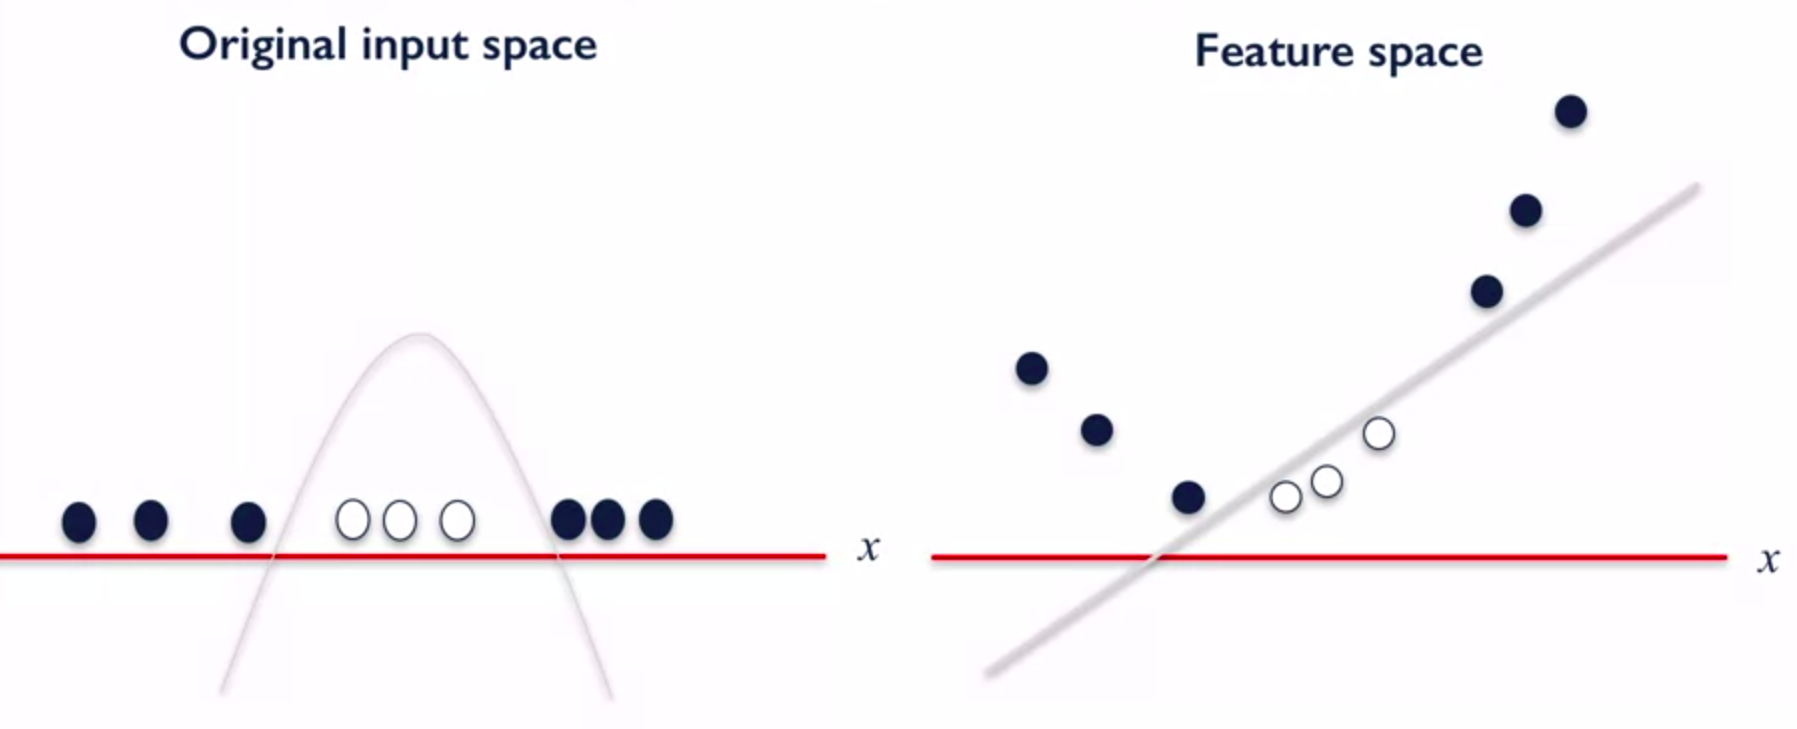
\includegraphics[scale=0.15]{kernel_2D.png}
\end{center}

\vspace{5mm}

From 2D to 3D:

\begin{center}
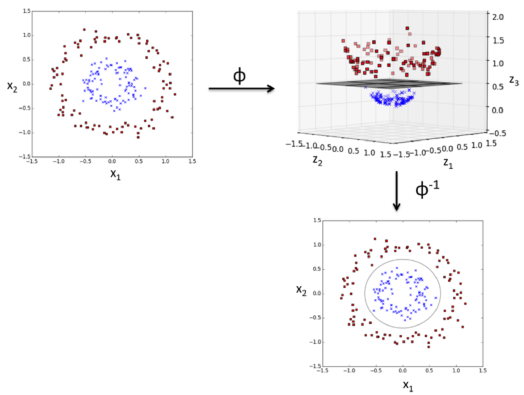
\includegraphics[scale=0.5]{kernel_3D.png}
\end{center}

\vspace{5mm}
{\fontsize{12pt}{22pt} \textbf{Neural network}\par}

\vspace{5mm}

\underline{Logistic regression with a neural network mindset}

Based on the example from coursera (\textit{deeplearning.ai})

Let us take the example of an image that we want to classify in a \textbf{binary} way: man/woman

The picture is vectorized as a vector of pixels : $\begin{pmatrix}x_1\\...\\x_p\end{pmatrix}$

We use a regression to predict if it's a man/woman:

$y=\omega^Tx + b$

Note: $x$ are all the pixels of \textbf{one} image.

\vspace{5mm}

We want a probability in output (if it's $\ge 0.5$ then we say it's a man).

We thus want the output to be $\widehat{y}=\sigma(\omega^Tx + b)=\mathbb{P}(y|x) \in [0,1]$

(see regression part to get more details on the sigmoid)

\vspace{5mm}

Now since it's a binary classification, we want the $y$ (real value) to be $0$ or $1$.

Thus, the loss function is:

$$\mathcal{L}(y, \widehat{y})=-y\log(\widehat{y})+(1-y)\log(1-\widehat{y})$$

\vspace{5mm}

The cost function is the empiric loss on all examples:

$$J(\omega, b)=\frac{1}{m}\Sigma_{i=1}^m\mathcal{L}(\widehat{y}^{(i)}, y^i)$$

\vspace{5mm}

\underline{Forward propagation}

$$x_1,x_2, \omega_1,\omega_p,b \to z=\omega_1x_1 + \omega_2x_2 + b \to \widehat{y}=a=\sigma(z) \to \mathcal{L}(a,y)$$

- First arrow: regression

- Second arrow: probability

- Third arrow: error

\vspace{5mm}

\underline{Backward propagation}

The idea is: with the error computed on the last step, we go backward in order to correct the parameters $\omega$ and $b$.

$$x_1,x_2, \omega_1,\omega_p,b \leftarrow z=\omega_1x_1 + \omega_2x_2 + b \leftarrow \widehat{y}=a=\sigma(z) \leftarrow \mathcal{L}(a,y)$$

Example: we want to find $\omega_1$ that minimizes the cost function:

$\frac{d\mathcal{L}}{d\omega_1}="d\omega_1"=\frac{d\mathcal{L}}{da}\frac{da}{dz}\frac{dz}{d\omega_1}=...=(a-y)x_1=dzx_1$

Steps:

We compute all the derivatives, then we apply the gradient descent

\lstset{language=Python}
\lstset{frame=lines}
\lstset{caption={Gradient descent (logistic regression with a NN mindset)}}
\lstset{label={lst:code_direct}}
\lstset{basicstyle=\footnotesize}
\begin{lstlisting}

for i in range(num_iterations):
        
     # Cost and gradient calculation
     grads, cost = propagate(w, b, X_train, Y_train) # propagation on ALL the training sample
        
     # Retrieve derivatives from grads
     dw = grads["dw"]
     db = grads["db"]
        
     # update parameters
     w = w - learning_rate * dw
     b = b - learning_rate * db
        
     # Record the costs
     costs.append(cost)

\end{lstlisting}

\lstset{language=Python}
\lstset{frame=lines}
\lstset{caption={Propagation (logistic regression with a NN mindset)}}
\lstset{label={lst:code_direct}}
\lstset{basicstyle=\footnotesize}
\begin{lstlisting}
def propagate(w, b, X, Y):
    
    m = X.shape[1]
    
    # FORWARD PROPAGATION (FROM X TO COST)
    A = sigmoid(np.dot(w.T,X)+b)
    cost = (- 1 / m) * np.sum(Y * np.log(A) + (1 - Y) * (np.log(1 - A))
    
    # BACKWARD PROPAGATION (TO FIND GRAD)
    dw = (1/m)*np.dot(X,(A-Y).T)
    db = (1/m)*np.sum(A-Y)

\end{lstlisting}



\vspace{5mm}
{\fontsize{12pt}{22pt} \textbf{AdaBoost}\par}

\vspace{5mm}

Boosting is an algorithmic paradigm addressing two major issues in machine learning:

- It optimizes the \hyperref[sec:bias-complexity-trade-off]{bias-complexity trade-off}. The learning starts with a basic class (large approximation error) and as it progresses the hypothesis class becomes more complex.

- It allows to find predictors that are usually computationally infeasible to find.

\vspace{5mm}

Main idea: weak learners are "boosted" to become stronger altogether.

\begin{center}
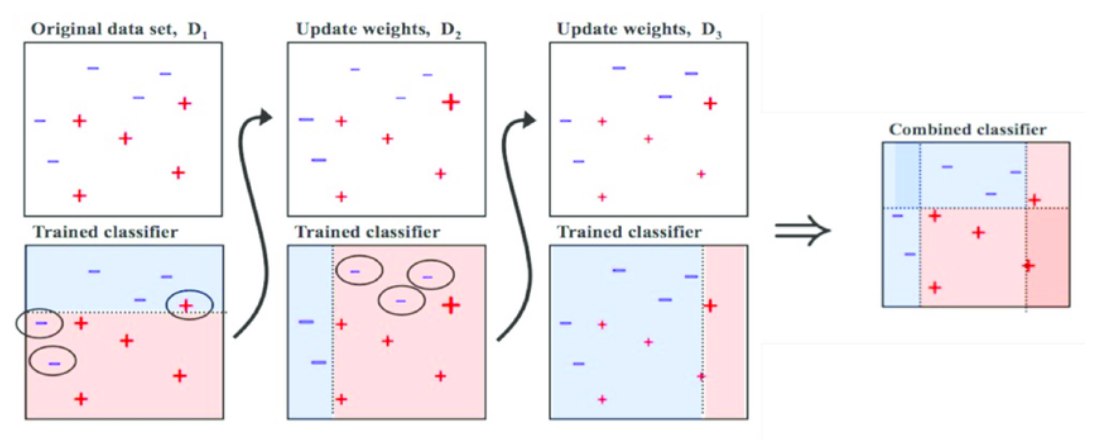
\includegraphics[scale=0.3]{AdaBoost_Schema.png}
\end{center}

Weak learner (or $\gamma$-weak-learner): it's an \textbf{algorithm} returning a function $h$ such that $L_{\mathcal{D}}(h) \leq 1/2 - \gamma$. In other words, it returns a simple binary predictor that does slightly better than a random guess.

\vspace{5mm}

\begin{algorithm}
\caption{AdaBoost}
\begin{algorithmic}
\State Input: training set $S=(x_1,y_1),...,(x_m,y_m)$, weak learner WL, number of rounds $T$
\State Initialize $D^{(1)} = (1/m,...,1/m)$ // same weights for all observations
\For{t = 1,...,T}
\State invoke weak learner $h_t = WL(D^{(t)},S)$
\State compute $\epsilon_t = \Sigma_{i=1}^m D_i^{(t)} \mathbbm{1}_{[y_i \neq h_t(x_i)]}$ // misclassification error
\State let $\omega_t = \frac{1}{2} log(\frac{1}{\epsilon_t}-1)$ // $\epsilon_t < 1$
\State update $D_i^{(t+1)} = \frac{D_i^{(t)} exp(-\omega_t y_i h_t(x_i))}{\Sigma_{j=1}^m D_j^{(t)} exp(-\omega_t y_j h_t(x_j))}$ for all $i=1,...,m$
\EndFor
\State Output: the hypothesis $h_s(x) = sign(\Sigma_{t=1}^T \omega_t h_t (x))$
\end{algorithmic}
\end{algorithm}

We note:

- Final predictor = weighted sum of weak predictors

- More weights are given to observations that gave wrong prediction. In doing so, the classifier of the next round will focus on these observations. Warning: to see this, focus on the variation of $D^{(t+1)}_i$ and not just $w_t$.

\vspace{5mm}

Theorem: the training error of the output hypothesis decreases exponentially fast with the number of boosting rounds.
{\fontsize{20pt}{22pt}\selectfont \textbf{Unsupervised learning} \par}
\vspace{10mm}
Unsupervised learning aims at \textbf{learning some underlying hidden structure of the data when we don't have the labels}.

\vspace{5mm}
{\fontsize{12pt}{22pt} \textbf{Expectation-Maximization (EM) in the case of GMM (Gaussian Mixture Model)}\par}

\vspace{5mm}

(for more details, see document \textit{gmm.pdf} in Cloud folder)

\vspace{5mm}

A GMM sample is composed of $j$ Gaussian variables (\textit{clusters}) distributed with proportions $(\pi_1,...,\pi_k)$ ($\Sigma \pi_i =1$)

We can write:

$$X \sim \mathcal{N}(\mu_{Z},\Sigma_{Z})~~~~~~with~~Z \sim \pi$$

$\pi$ is not really a law but more the proportions of each Gaussian categories.

Thus, $X$ has a density which is a weighted-average of all Gaussian densities:

$$p_\theta(x) = \Sigma_{j=1}^{k}\pi_j f_j(x)~~~~~~~(*)$$


\underline{Estimation}

We want to estimate $\theta = (\pi, \mu, \Sigma)$ where:

$\pi=(\pi_1,...,\pi_k)$, $\mu=(\mu_1,...,\mu_k)$, $\Sigma=(\Sigma_1,...,\Sigma_k)$

\vspace{5mm}

To do so, we use the maximum likelihood method (product of densities across all samples):

$$p_\theta(x)=\Pi_{i=1}^n p_\theta(x_i)$$

$$l(\theta)=log(\Pi_{i=1}^n p_\theta(x_i))=\Sigma_{i=1}^n log(p_\theta(x_i))$$

We thus need to find $argmax(l(\theta))$

Problem: the likelihood function is not convex!

\vspace{5mm}

The expectation-maximization problem is used when we have \textit{latent variables} (= variables for which we don't know their associated distribution).

Let $z=(z_1,...,z_k)$ be the vector of latent variables. We can express the density $(*)$ as a joint function with respect to $z$:

$$p_\theta(x,z)=p_\theta(z)p_\theta(x|z)$$

$$l(\theta, z) = ... =\Sigma(log \pi_{z_i})+ \Sigma(logf_{z_i}(x_i))$$

A classic optimization (in case of Gaussians) give us empirical values as solutions e.g. $\hat{\pi_j}=\frac{n_j}{n}$

Problem: we don't know $j$!

\vspace{5mm}

We will thus use the \textit{expected} log-likelihood method.

Let us find another expression of the likelihood:

$$p_\theta(x,z)=p_\theta(x)p_\theta(z|x)$$

As seen previously: $p_\theta(x,z)=\Pi \pi_{z_i}f_{z_i}(x_i)$

$p_\theta(z|x)=\Pi p_\theta(z_i|x_i)=\frac{\Pi \pi_{z_i}f{z_i}(x_i)}{p_\theta(x_i)} \propto \Pi \pi_{z_i}f{z_i}(x_i)$

\vspace{5mm}

Given an initial parameter $\theta_0$, the \textit{expected} log-likelihood is written as such:

$$\mathbb{E}_{\theta_0}[l(\theta;z)]=\Sigma p_{\theta_0}(z|x) l(\theta;z)$$
$$\mathbb{E}_{\theta_0}[l(\theta;z)]=\Sigma_{j} \Sigma_{i} p_{ij}(log\pi_j+logf_j(x_i))$$

We now have an expression that doesn't depend on $z$ but only on $p_{ij}$ and we know that $n_j=\Sigma_i p_{ij}$

\vspace{5mm}
{\fontsize{12pt}{22pt} \textbf{K-means}\par}

\vspace{5mm}

(see kmeans.pdf from OneDrive folders for more details)

\vspace{5mm}

Objective: group data into $k$ clusters so that samples in the same cluster are close to each other w.r.t. the Euclidean distance.

\vspace{5mm}
The cost function minimization is written as such:

$$\underset{C_1,...,C_k;\mu_1,...,\mu_k}{\operatorname{argmin}}\Sigma_{j=1}^k\Sigma_{i \in C_j}||x_i-\mu_j||^2$$

Where $\mu_j$ is the mean, also called gravity center or cluster center:

$$\mu_j=\frac{1}{|C_j|}\Sigma_{i \in C_j}x_i$$

\begin{algorithm}
\caption{K-means}
\begin{algorithmic}
\State Input: $x_1,...,x_n$
\State Output: clusters $C_1,...,C_k$
Random values for $\mu_1,...,\mu_k$
\While{no convergence}
\State // Step 1: Update clusters
\State $C_1,...,C_k \leftarrow \emptyset$
\For{$i=1$ to $n$}
\State $j \leftarrow argmin_l ||x_i - \mu_l||$
\State $C_j \leftarrow C_j + \{i\}$ // We add observation $i$ to the cluster $C_j$
\EndFor
\State // Step 2: Update cluster centers
\For{$j=1$ to $k$}
\State $\mu_j \leftarrow 0$
\State $n_j \leftarrow 0$
\For{$i$ in $C_j$} // We loop on all observations of each cluster
\State $\mu_j \leftarrow \mu_j + x_i$
\State $n_j \leftarrow n_j +1$
\EndFor
\State $\mu_j \leftarrow \mu_j /n_j$
\EndFor
\EndWhile
\end{algorithmic}
\end{algorithm}

The quality of the clustering strongly depends on the initial center values. This is why the algorithm is generally run multiple times for different initial values. The best clustering (i.e., that of minimum cost) is returned.

\vspace{5mm}

\underline{K-means++}

To improve the quality of the clustering, we choose the initial cluster centers far from each other:

- select the first cluster center uniformly at random among the n data samples

- select the following cluster centers at random, with a probability proportional to the square distance to the closest current cluster center

\lstset{language=Python}
\lstset{frame=lines}
\lstset{caption={K-means++ initial centers selection}}
\lstset{label={lst:code_direct}}
\lstset{basicstyle=\footnotesize}
\begin{lstlisting}

centers = []
centers.append(X[np.random.randint(X.shape[0])]) # inital center = one random sample
distance = np.full(X.shape[0], np.inf) # a vector (n,1) with only infinity terms
for j in range(1,self.n_clusters):
    distance = np.minimum(np.linalg.norm(X - centers[-1], axis=1), distance) # size (n,1); 
# distance = the smallest distance associated with 
# the last added center
    p = np.square(distance) / np.sum(np.square(distance)) # probability vector [p1,...,pn]
# the highest probability in p is associated 
# with the biggest distance w.r.t the last added center
    sample = np.random.choice(X.shape[0], p = p) # one sample is 
						 # selected according to probabilities
    centers.append(X[sample])

\end{lstlisting}

\textcolor{gray}{Note: this problem is called \textit{NP-hard problem}. It means that its complexity is at least equal to the complexity of an NP-problem}

\textcolor{gray}{NP-problem: a problem is NP if it can be determined by a non-deterministic Turing machine in polynomial time. Intuitively, a problem is NP if we can quickly verify if one candidate is a solution of the problem. E.g. "travelling salesman problem" = let $d$ be a distance and $n$ be a number of cities. Is there an itinerary with distance $\ge d$ stopping by every city? -> easy to check...}

\vspace{5mm}
\textcolor{gray}{Turing machine (1936)}

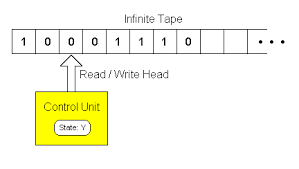
\includegraphics{../images/turingmachine.png}

\textcolor{gray}{"non-deterministic turing machine": itinerary can be represented by a tree...}

\vspace{5mm}


{\fontsize{12pt}{22pt} \textbf{Local Outlier Factor}\par}

\vspace{5mm}

Local Outlier Factor is an unsupervised method used in anomaly detection. It consists of comparing local density of train observations VS local density of test observations. \\

\underline{Reachability distance} \\

$reachability \mbox{-} distance_k(A,B) = max \{ k \mbox{-} distance (B), d(A,B)\}$  = reachability of A \textit{from} B. \\

$k \mbox{-} distance (B)$: distance from B to its kth nearest neighbor.

The reachability distance of A from B is \textit{at least} the distance between A and B or \textit{at least} the distance of B's neighbor.

When A is very far from B, it's simply the distance between the two points.

When A is very close to B, it's the distance between B and its neighbor. \\

The distance can be computed using different metrics: Euclidean distance, Mahalanobis distance, etc. \\

\underline{Local reachability density} \\

$lrd_k (A) = \frac{1}{\Sigma_{B \in N_k(A)} reachability \mbox{-} distance_k(A,B) / |N_k(A)|}$ \\

It's the inverse of the average of reachability-distances of A from B.

When A is very far from its neighbors: sum of reachability distances is high => local reachability density is small. \\

\underline{Local Outlier Factor} \\

LOF computation consists of comparing the local densities of a point VS its neighbors. \\

$LOF_k(A) : =  \frac{\frac{\Sigma_{B \in N_k(A)}lrd_k(B)}{lrd_k(A)}}{|N_k(A)|}$ \\

$LOF_k(A) > 1$: A is an outlier. Local reachability density of A is small compared to its neighbors.

$LOF_k(A) < 1$: A is an inlier.

\begin{center}
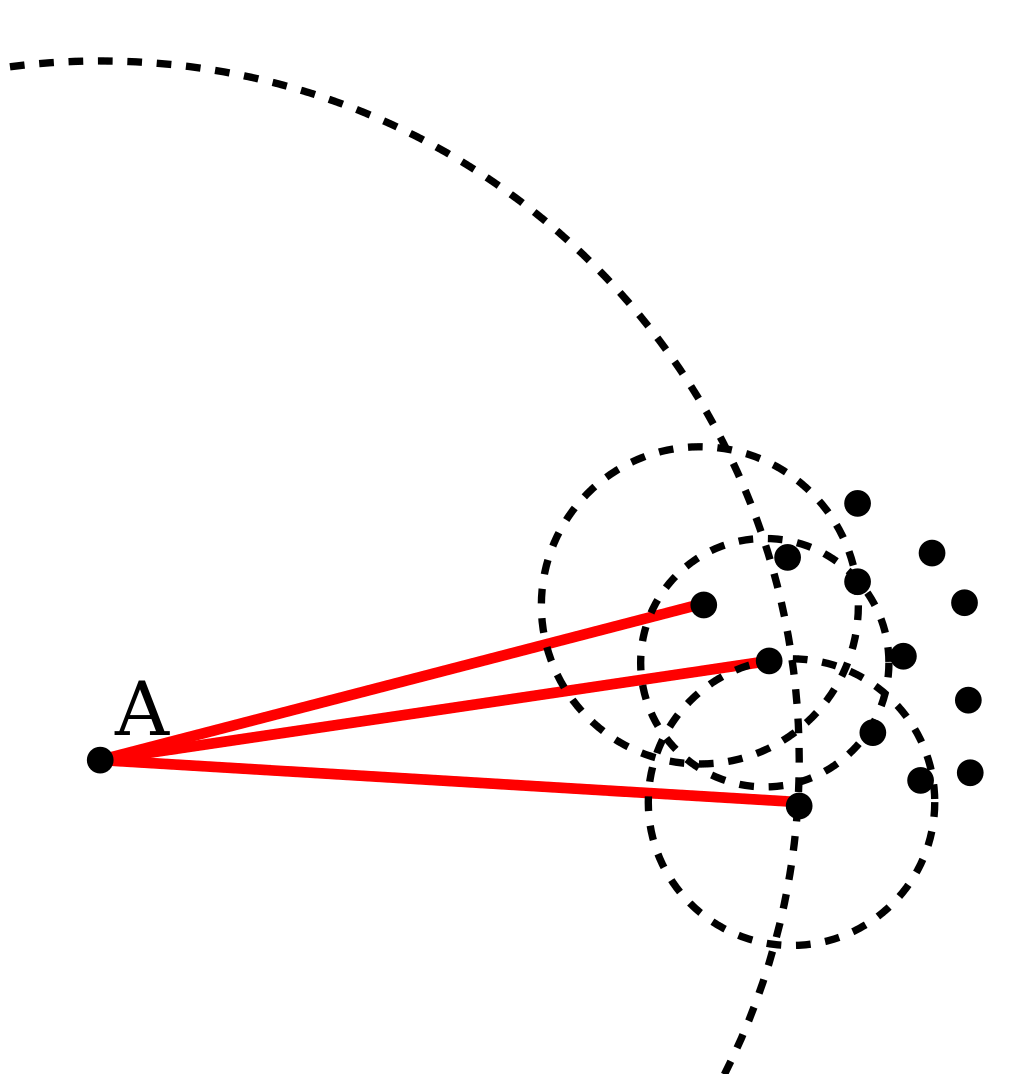
\includegraphics[scale=0.10]{LOF.png}
\end{center}

On this figure, $k = 3$. We can see that the reachability distance of A from its neighbors is high (red segments). The local reachability density of A will thus be \textbf{low}.

On the contrary, the local reachability densities of its neighors is \textbf{high} because each neighbor can be easily reached from their own neighbors.

As a result, LOF would be high so A is an outlier. \\

\underline{sklearn algorithm} \\

To score an observation, \textit{fit} simply memorizes the train observations (same as in knn). 

\textit{score\_samples} first finds the k-nearest neighbors from the train set thanks to the given distance metric. It then computes the local outlier factor for each test observation comparing the test observation local density with its closest k-neighbors local densities in the train set.

\vspace{5mm}
{\fontsize{12pt}{22pt} \textbf{Variational Auto-Encoder}\par}

\vspace{5mm}

Variational autoencoders are a combination of three things:

1. Autoencoders

2. Variational Approximation \& Variational Lower Bound

3. "Reparameterization" Trick

\vspace{5mm}

1. Autoencoders

Autoencoders are used to extract features from unlabeled training data. They are new methods for \textbf{dimensionality reduction} and part of neural networks branch.

\vspace{5mm}

\textit{Note}: autoencoders can be used to replace older dimensionality reduction methods such as PCA for several reasons:

- For very large data sets that can’t be stored in memory, PCA will not be able to be performed. The autoencoder construction using keras can easily be batched resolving memory limitations.

- PCA is restricted to linear separation while autoencoders are capable of modelling complex non linear functions.

\begin{center}
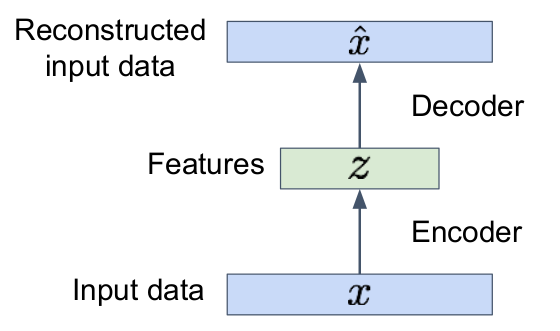
\includegraphics[scale=0.3]{Autoencoders.png}
\end{center}

\vspace{5mm}

Learning can be done using a loss function such as $||x - \widehat{x}||^2$. In a similar way than neural network, optimization is typically done with backpropagation.

\vspace{5mm}

2. Variational Approximation \& Variational Lower Bound

\vspace{5mm}

We assume $x$ is generated from unobserved (latent) $z$:

\begin{center}
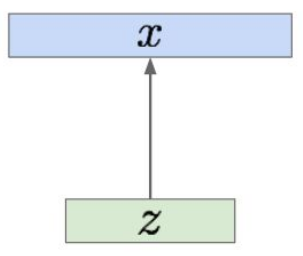
\includegraphics[scale=0.3]{decoder.png}
\end{center}

\vspace{5mm}

\textit{Practical example}: $x$ can be seen as images and $z$ as the main attributes (orientation, colors, etc.)

\vspace{5mm}

$x \sim p_{\theta^*}(x | z)$ where $p_{\theta^*}(x | z)$ is called \textit{true conditional}

$z \sim p_{\theta^*}(z)$ where $p_{\theta^*}(z)$ is called \textit{true prior}

\vspace{5mm}

Objective: estimating $p_{\theta}(x)$. We thus need to estimate $\theta^*$.

\vspace{5mm}

We can do it through maximum likelihood. The marginal density is $p_{\theta}(x) = \int p_{\theta}(x|z) p_{\theta}(z) dz$

\vspace{5mm}

\textit{Note}: a marginal likelihood function is a likelihood function in which some parameter variables have been marginalized. Marginalization consists in summing over the possible values of one variable in order to determine the contribution of another. E.g., $\mathbb{P}(X)=\Sigma_y \mathbb{P}(X, Y=y)$ or in continuous probabilities $p(x)=\int p(x, y) dy$. Also, if we don't know the joint probability, we can express this using conditional probabilities: $p(x)=\int p(x | y) p(y) dy$

\vspace{5mm}

Problem: impossible to compute $p(x|z)$ for every $z$ (\textcolor{orange}{computationally too expensive}) => problem is said \textbf{intractable}

\vspace{5mm}

Solution: use another encoder learning $q_\phi (z|x)$ that approximates $p_\theta(z | x)$

\begin{center}
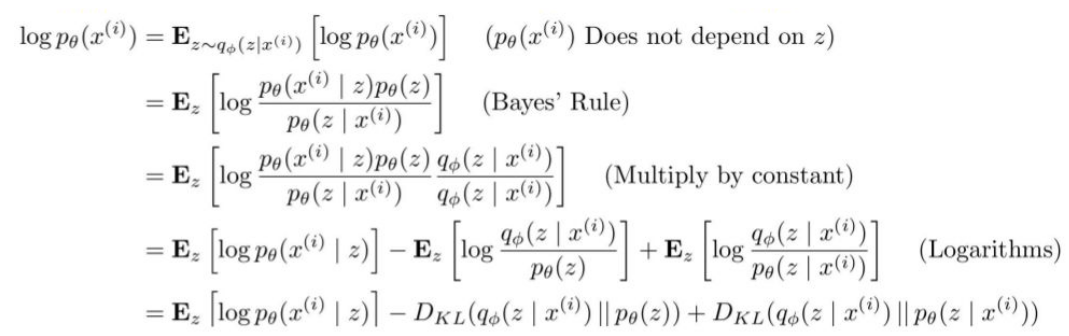
\includegraphics[scale=0.4]{log-likelihood-VAE.png}
\end{center}

\vspace{5mm}

$\mathbb{E}_z[\log p_\theta (x^{(i)} | z]$: we can estimate this term through sampling

$D_{KL}(q_\phi(z | x^{(i)}) || p_\theta(z))$: differentiable term

$D_{KL}(q_\phi(z | x^{(i)}) || p_\theta(z | x^{(i)}))$: $p(z|x)$ intractable but we know that $D_{KL} \geq 0$

\vspace{5mm}

Let $\mathcal{L}(x^{(i)}, \theta, \phi) = \mathbb{E}_z[\log p_\theta (x^{(i)} | z] - D_{KL}(q_\phi(z | x^{(i)}) || p_\theta(z))$ = \textbf{tractable lower bound} that we can optimize

\vspace{5mm}

We know that $p_\theta (x^{(i)}) \geq \mathcal{L}(x^{(i)}, \theta, \phi)$ since $D_{KL}(q_\phi(z | x^{(i)}) || p_\theta(z | x^{(i)})) \geq 0$

Thus the maximum likelihood problem becomes: $\theta^*, \phi^* = argmax_{\theta, \phi} \Sigma_{i=1}^N \mathcal{L}(x^{(i)}, \theta, \phi)$

\vspace{5mm}

We can minimize $D_{KL}(q_\phi(z | x^{(i)}) || p_\theta(z))$ making posterior distribution close to prior. To do so, we make encoder network predicting $\mu_{z | x}$ and $\Sigma_{z | x}$ and then we sample $z | x \sim \mathcal{N}(\mu_{z | x}, \Sigma_{z | x})$

\begin{center}
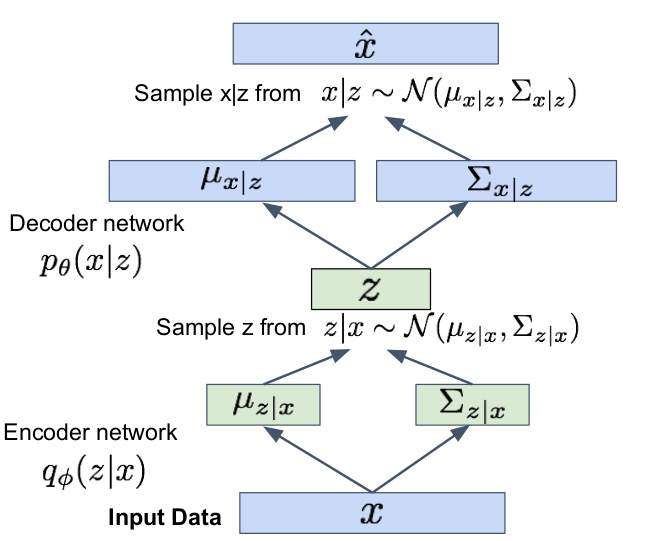
\includegraphics[scale=0.4]{VAE_final_schema.png}
\end{center}

Problem: sampling $z | x \sim \mathcal{N}(\mu_{z | x}, \Sigma_{z | x})$ and $x | z \sim \mathcal{N}(\mu_{x | z}, \Sigma_{x | z})$ is not differentiable (\textcolor{orange}{why?}).

=> we use \textbf{reparametrization trick}: we sample $z_0 \sim \mathcal{N}(0,1)$ to have $z = \mu_{x | z} + z_0 \Sigma_{x | z} \sim \mathcal{N}(\mu_{x | z}, \Sigma_{x | z})$

\begin{center}
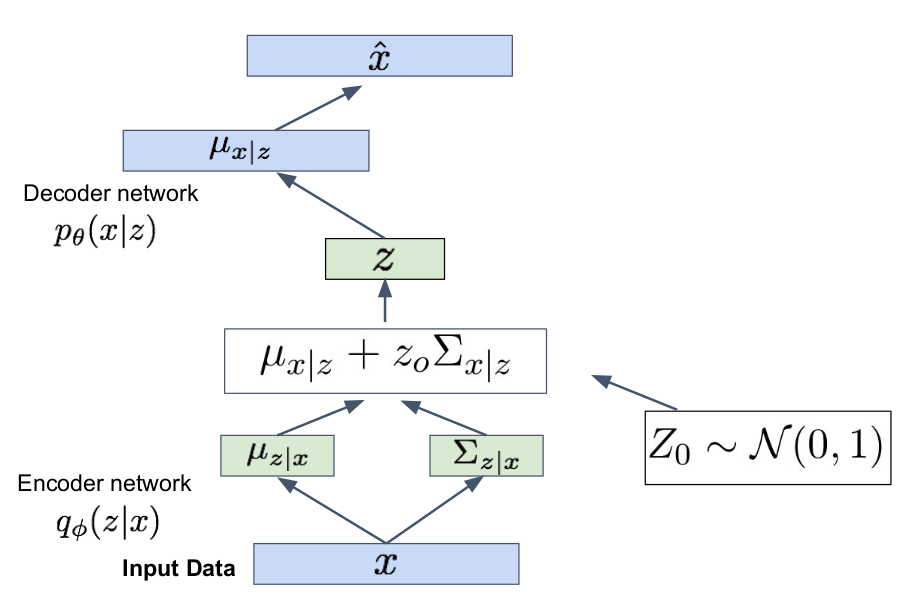
\includegraphics[scale=0.4]{VAE_reparametrization_trick.png}
\end{center}

Optimization through forward and backward propagation!
\vspace{10mm}
{\fontsize{20pt}{22pt}\selectfont \textbf{Reinforcement learning} \par}
\vspace{10mm}
Reinforcement learning is inspired on human logic: we learn which strategy to take thanks to rewards we receive.

\vspace{5mm}

Reinforcement learning uses Markov Decision Processes (MDP).

A Markov Decision Process is defined by:

- an initial state $s_0$

- the reward distribution $r_t \sim p(r | s_t, a_t)$ (stochastic)

- the transition probabilities, $s_{t+1} \sim p(s | s_t, a_t)$ (stochastic)

=> \textbf{MDP: we know the state and the reward from the previous state only}.

\vspace{5mm}

A \textit{policy} is an action for each state, for a given MDP.

=> \textbf{a policy can be seen as a strategy: we know where to go at each state}. In practice the policy is actually the \textbf{transition probability matrix}.

\vspace{5mm}

The \textit{value function} is the gain we earn at a state, for a specific policy: $\forall s, V_\pi(s) = \mathbb{E}_{\pi}[G | s_0 = s]$

=> \textbf{The expected gain takes into account the transition probability.}

The gain is calculated as such: $G = r_0 + \gamma r_1 + \gamma^2 r_2 +... = \Sigma_t \gamma^t r_t $ where $\gamma$ is the \textit{discount factor}.

$V$ can also be written $V_\pi(s) = \mathbb{E}_\pi[r_0 + \gamma V(s_1) | s_0 = s]$. This expression is called \textbf{Bellman equation}.

\vspace{5mm}

We can find the best policy:

$\forall s, \pi^*(s) = a^* \in argmax_a\mathbb{E}_\pi[r_0 + \gamma V_*(s_1) | s_0 = s, a_0 = a]$

Where $V_*$ is solution of the \textbf{Bellman optimality equation}:

$\forall s, V(s) = max_a\mathbb{E}[r_0 + \gamma V(s_1) | s_0 = s]$

\vspace{5mm}
{\fontsize{12pt}{22pt} \textbf{Online estimation}\par}

\vspace{5mm}

The expected value function is approached using empiric estimator (sum).

Two ways to do it:

- Monte-Carlo update: if we can memorize all the paths, we update the sum at each step $S \leftarrow x_t$. At the end we compute the mean $X \leftarrow \frac{S}{t}$

- TD-learning: we update the value function using temporal differences $\forall s, V(s_t) \xleftarrow{\alpha} r_t + \gamma V(s_{t+1})$

Where $X \xleftarrow{\alpha} x_t <=> X = X + \alpha (x_t - X)$ ($\alpha$ is usually $1/t$)

\vspace{5mm}
{\fontsize{12pt}{22pt} \textbf{Online control}\par}

\vspace{5mm}

Recall that value function is $\forall s, V_\pi(s) = \mathbb{E}[G | s_0 = s]$

Unknown model <=> "unknown strategy" <=> we don't know the rewards in advance (we need to learn \textit{online}).

=> we cannot compute the expectation $\mathbb{E}$

=> instead of the value function, we will estimate the \textbf{value-action function} thanks to the Bellman equation:

\begin{center}
$\forall s, a,~~~~~Q_\pi(s,a) = \mathbb{E}_\pi[r_0 + \gamma Q(s_1, a_1) | s_0 = s, a_0 = a]$
\end{center}

=> for an initial state and a fixed action, we can compute the $Q$ function

=> the value-action function can be seen as the expected (=> use of transition matrix (probabilities)) gain we get at a state when doing a specific action

\textit{Note}: the policy $\pi$ takes account only from next state $s_1$

\vspace{5mm}

We want to \textit{control} the policy and find the optimal one: $\pi^*(a) = a^* \in argmax_a Q_*(s,a)$

\vspace{5mm}

The optimal Bellman equation becomes:

\begin{center}
$\forall s, a,~~~~~Q_\pi(s,a) = \mathbb{E}_\pi[r_0 + \gamma max_{a'} Q(s_1, a') | s_0 = s, a_0 = a]$
\end{center}

How to choose initial state $a_0$?

--> Pure exploitation: we find the best action knowing the current system $\pi(s) \leftarrow argmax_a Q(s,a)$

=> problem: $Q$ is estimated, thus we have a chance to miss good actions

--> Pure exploration: $\pi(s) \leftarrow random$

=> problem: we can waste time on bad actions and thus have bad estimation quality

Solution: trade-off  exploitation/exploitation (SARSA, Q-learning, ...).

\vspace{5mm}
\underline{SARSA}

\vspace{5mm}

This algorithm is based on $\epsilon$-greedy algorithm.

  \begin{equation}
 \pi(s) \leftarrow
    \begin{cases}
     a^* \in argmax_a Q(s,a) $ with probability $ 1-\epsilon \\
    random $ with probability $ \epsilon
    \end{cases}
  \end{equation}

=> with a small probability ($\epsilon$ is usually lower than $5\%$), we do random actions. Otherwise we take the best action of the known ones.

\vspace{5mm}

\textbf{Estimation} is done through \textit{TD-learning} (temporal differences - see Online Estimation):

\begin{center}
$\forall t, Q(\textcolor{blue}{s}_t, \textcolor{blue}{a}_t) \xleftarrow{\alpha} \textcolor{blue}{r}_t + \gamma Q(\textcolor{blue}{s}_{t+1}, \textcolor{blue}{a}_{t+1})$
\end{center}

\lstset{language=Python}
\lstset{frame=lines}
\lstset{caption={SARSA}}
\lstset{label={lst:code_direct}}
\lstset{basicstyle=\footnotesize}
\begin{lstlisting}

# action is identified with new state (after move) except teleportation (action = same state)

def sarsa(Q, model = model, alpha = 0.1, eps = 0.1, n_iter = 100):
    states = model.states
    terminals = model.terminals
    rewards = model.rewards
    gamma = model.gamma
    # random state (not terminal)
    state = np.random.choice(np.setdiff1d(np.arange(len(states)), terminals))
    # random action
    action = np.random.choice(Q[state].indices)
    new_state = action
    for t in range(n_iter):
        state_prev = state
        action_prev = action
        state = new_state
        if state in terminals: # if the new action gives terminal state
            	# we start again from a new random state
	            state = np.random.choice(np.setdiff1d(np.arange(len(model.states)),
									 terminals))
	            action = np.random.choice(Q[state].indices)
	            Q[state_prev, action_prev] = 
		(1 - alpha) *  Q[state_prev, action_prev] + alpha * rewards[action_prev]
		  # we removed the second term since state_prev was the last step
        else:
		  # we choose the best action that has the highest expected value-action
	            best_action = Q[state].indices[np.argmax(Q[state].data)]
	            if np.random.random() < eps: 
		# with probability of epsilon, we choose a random action
	                action = np.random.choice(Q[state].indices)
	            else:
	                action = best_action
	            Q[state_prev, action_prev] = 
			(1 - alpha) *  Q[state_prev, action_prev] 
			+ alpha * (rewards[action_prev] + gamma * Q[state, action])
        new_state = action
    return Q

\end{lstlisting}

\vspace{5mm}
\underline{Q-learning}

\vspace{5mm}

This algorithm is also based on $\epsilon$-greedy algorithm.

  \begin{equation}
 \pi(s) \leftarrow
    \begin{cases}
     a^* \in argmax_a Q(s,a) $ with probability $ 1-\epsilon \\
    random $ with probability $ \epsilon
    \end{cases}
  \end{equation}

\textbf{Estimation}: unlike SARSA, Q-learning aims at updating the estimator using the best action at each iteration:

\begin{center}
$\forall t, Q(s_t, a_t) \xleftarrow{\alpha} r_t + \gamma max_{a} Q(s_{t+1}, a)$
\end{center}

The only modification from SARSA is the following line:

\lstset{language=Python}
\lstset{frame=lines}
\lstset{caption={Q-Learning}}
\lstset{label={lst:code_direct}}
\lstset{basicstyle=\footnotesize}
\begin{lstlisting}
Q[state_prev, action_prev] = (1 - alpha) *  Q[state_prev, action_prev] 
			+ alpha * (rewards[action_prev] + gamma * np.max(Q[state].data))
\end{lstlisting}

\vspace{5mm}
\end{document} 
